\documentclass{article}

\usepackage[margin=1in]{geometry}
\usepackage{graphicx} % Allow image/pdf includes
\usepackage{extramarks} % Extra header marks (continued on next page)
\usepackage{amsmath} % Math enhancements
\usepackage{amsthm} % Theorem typesetting
\usepackage{amssymb} % Extended symbol collection
\usepackage{tikz} % Graphical element creation
\usetikzlibrary{automata,positioning}
\usepackage{algpseudocode} % Algorithm layout
\usepackage{enumitem} % Enumerate (lists)
\usepackage{ragged2e} % Alternative alignment
\usepackage{gensymb} % Generic symbols (degree, etc)
\usepackage{empheq} % Allow \boxed around \begin{empheq}
\usepackage{color,soul} % Highlighting
\usepackage{booktabs} % Enhanced table creation
\usepackage{multirow} % Table multi row
\usepackage{mathtools} % Math enhancements
\usepackage{bm} % Bold math
\usepackage[mathscr]{euscript} % Script variables
\usepackage{cancel} % Cancel through text
\usepackage{color,soul} % Highlighting
\usepackage{mathtools}
\usepackage{multirow}
\usepackage{mathrsfs}
\usepackage{physics}
\usepackage{gensymb}
\usepackage{siunitx}
\usepackage{subcaption}
\usepackage[]{algorithm2e}
\usepackage{float}
\usepackage[cache=false]{minted}
\renewcommand{\MintedPygmentize}{/Users/loganharbour/miniconda/bin/pygmentize}
\usepackage[scaled]{beramono}
\usepackage[T1]{fontenc}
\usepackage{diagbox}

\setlength\parindent{0pt} % No indents
\setlength{\parskip}{1em} % Paragraph skip

\newcommand{\vx}{\mathbf{x}} % x vector
\newcommand{\vy}{\mathbf{y}} % x vector

\newcommand{\pageTitle}{MEEN 644 - Homework 4}
\newcommand{\pageAuthor}{Logan Harbour}

\begin{document}

\title{\LARGE \textbf{\pageTitle} \vspace{-0.3cm}}
\author{\large \pageAuthor}
\date{\vspace{-0.6cm} \large \today \vspace{-0.4cm}}

\maketitle

\section{Problem statement}

\begin{center}
	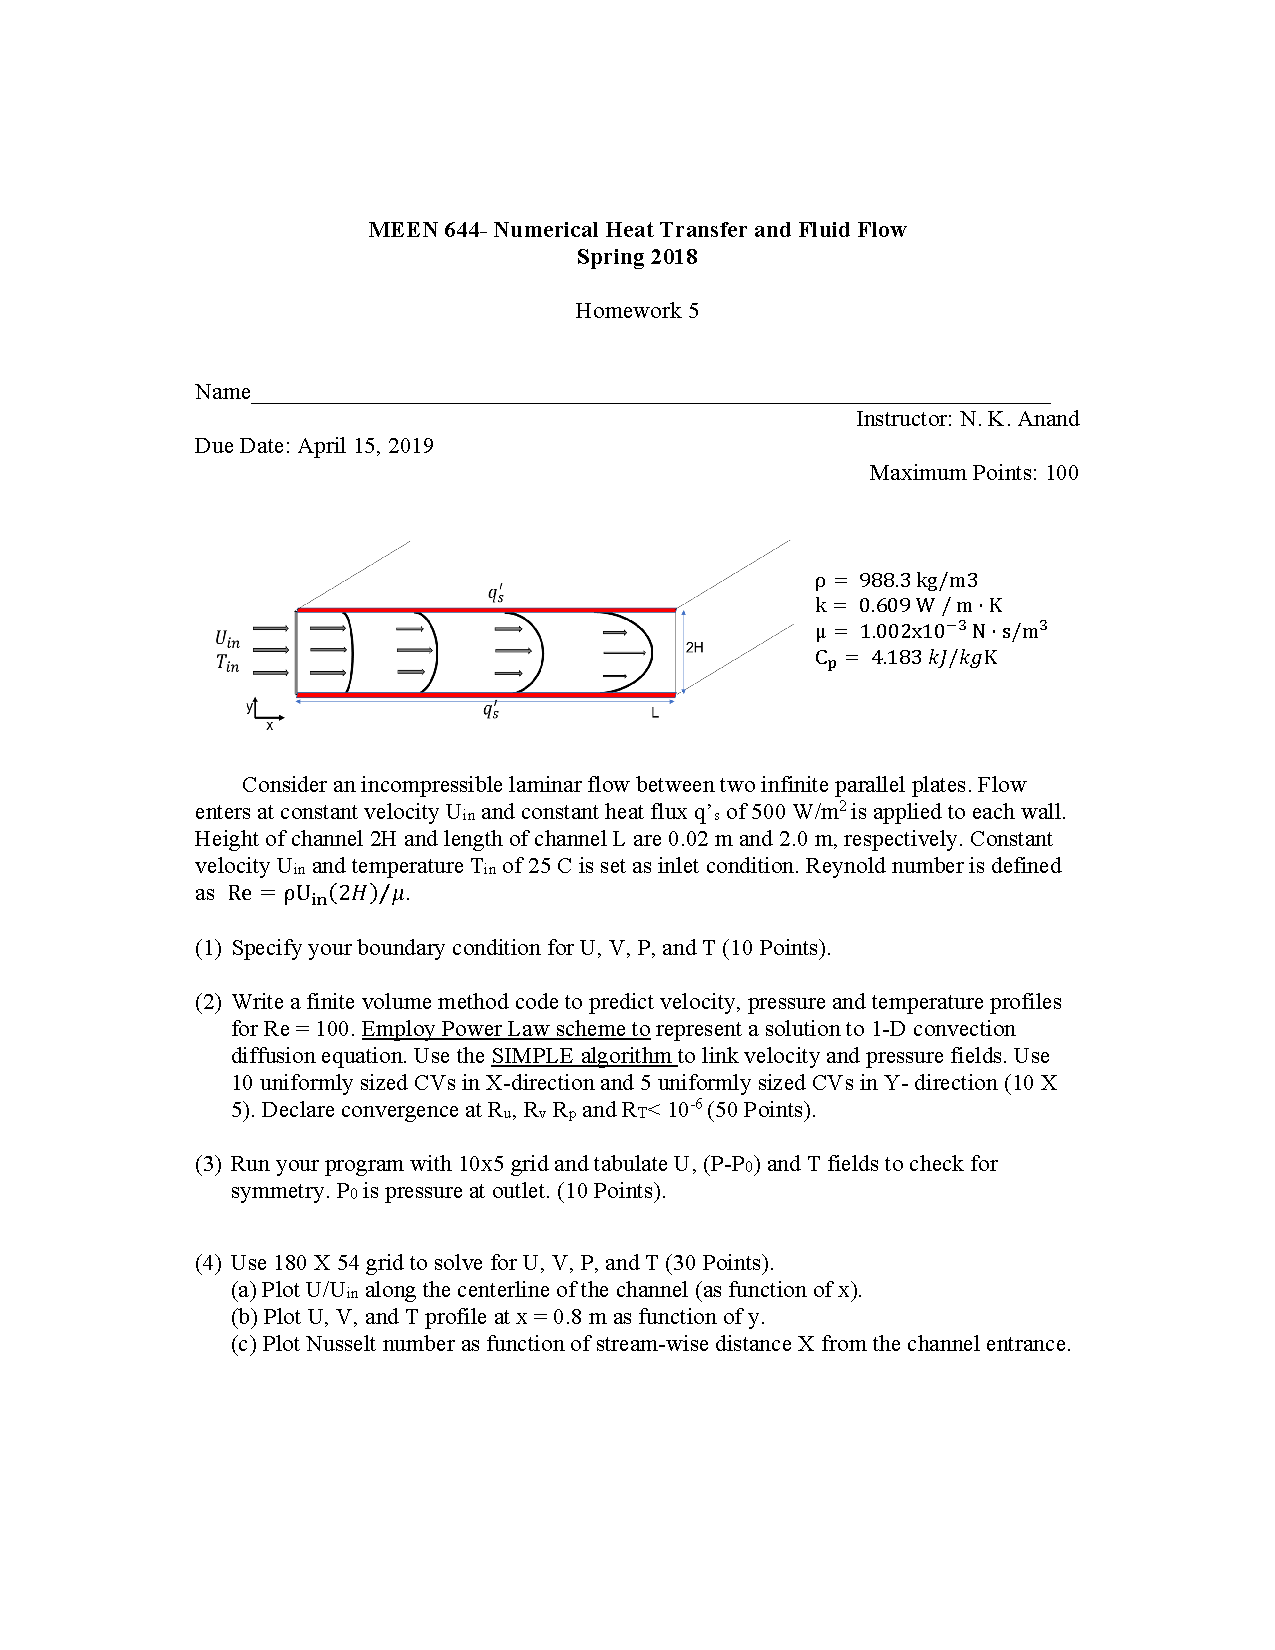
\includegraphics[trim={3.6cm 15.5cm 4cm 9.0cm},clip,page=1,scale=0.8]{../doc/hwk5.pdf}
\end{center}

Consider an incompressible laminar flow between two infinite parallel plates. Flow enters at constant velocity $u_\mathrm{in}$ and aconstant heat flux, $q' = 500$ W/m$^2$ is applied to each wall. Height of channel $2H$ and length of channel $L$ are 0.02 m and 2.0 m, respectively. Constant velocity $u_\mathrm{in}$ and temperature $T_\mathrm{in} = 25^\circ$C is set as the inlet condition. Reynolds number is defined as $Re = 2 \rho u_\mathrm{in} H / \mu$.
\begin{enumerate}
	\item \textbf{(10 points)} Specify your boundary condition for $u, v, P,$ and $T$.
	\item \textbf{(50 points)} Write a finite volume method code to predict velocity, pressure, and temperature profiles for Re = 100. Employ the Power Law scheme to represent a solution to a 1-D convection-diffusion equation. Use the SIMPLE algorithm to link velocity and pressure fields. Use 10 uniformly sized CVs in the $x$-direction and 5 uniformly sized CVs in the $y$-direction. Declare convergence at $R_u, R_v, R_P$ and $R_T < 10^{-6}$. 
	\item \textbf{(10 points)} Run your program with the 10 $\times$ 5 grid and tabulate $u, (P - P_0)$, and $T$ to check for symmetry. $P_0$ is the pressure at the outlet.
	\item \textbf{(30 points)} Use a $180 \times 54$ grid to solve for $u, v, P,$ and $T$.
	\begin{enumerate}[label=(\alph*)]
		\item Plot $u/u_\mathrm{in}$ along the centerline of the channel (as a function of $x$).
		\item Plot $u, v,$ and $T$ at $x = 0.8$m m (as a function of $y$).
		\item Plot the Nusselt number as a function of stream-wise distance $x$ from the channel entrance.
	\end{enumerate}
\end{enumerate}

\section{Preliminaries}

\subsection{Two-dimensional diffusion-convection}

With two-dimensional diffusion and convection with constant material properties, we have the PDE
\begin{equation}
\begin{cases}
\pdv{u}{x} + \pdv{v}{y} = 0\,,\\
\rho u \pdv{u}{x} + \rho v \pdv{v}{x} = - \pdv{P}{x} + \mu \pdv{^2u}{x^2} + \mu \pdv{^2u}{y^2}\,,\\
\rho u \pdv{u}{y} + \rho v \pdv{v}{y} = - \pdv{P}{y} + \mu \pdv{^2v}{x^2} + \mu \pdv{^2v}{y^2}\,.
\end{cases}
\label{eq:diffusionconvection}
\end{equation}
with the boundary conditions
\begin{equation}
\begin{cases}
u(x, L_y) = 0\,, \\
\pdv{^2u}{x^2} \big|_{(L_x, y)} = 0 \,, \\
u(x, 0) = 0 \,, \\
u(0, y) = \frac{\mathrm{Re} \mu}{\rho L_y} \,, \\
v(x, L_y) = 0\,, \\
v(L_x, y) = 0 \,, \\
v(x, 0) = 0\,, \\
v(0, y) = 0 \,,
\end{cases}\,.
\end{equation}

\subsection{Solving methodology}

Using the SIMPLE algorithm, the problem is solved in the following order:
\begin{enumerate}
	\item Explicitly fill the boundary conditions into the $u$ and $v$ solution vector in order to enforce them in all of the integrations that follow.
	\item Guess a pressure field, $p^*$.
	\item Use the guessed (or previously iterated) pressure field to obtain the velocity guesses, $u^*$ and $v^*$, as discussed in \ref{subsec:velocity-guess}.
	\item Solve the pressure correction, $p'$, as discussed in \ref{subsec:pc-solve}.
	\item Compute the velocity corrections, $u'$ and $v'$, and correct the velocity and pressure field, as discussed in \ref{subsec:correction}. 
	\item Correct for the $u$-velocity outflow boundary condition.
	\item Check for convergence. If not converged, return to 2.
	\item Solve the auxiliary temperature until convergence.
\end{enumerate}

\subsection{Domain discretization}

The domain of size $L_x \times L_y$ is discretized into $N_x \times N_y$ uniformly sized control volumes with $\Delta x = L_x / N_x$ and $\Delta y = L_y / N_y$. The numbering for all variables begins at the origin at $(i, j) = (0, 0)$. The maximum index for each variable, $\phi$, is defined as $(M_x^\phi, M_y^\phi)$.

\begin{figure}[H]
	\centering
	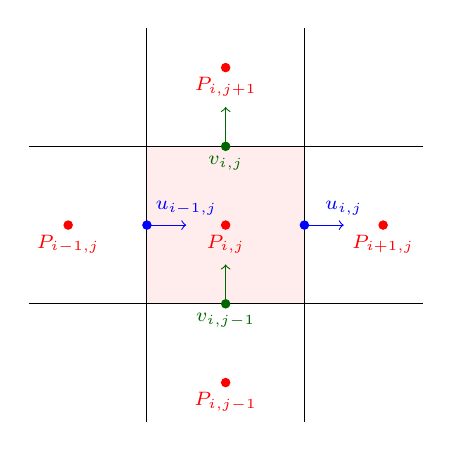
\begin{tikzpicture}[scale=1, style={font=\scriptsize}]
	\tikzset{dimen/.style={<->,>=latex,thin,every rectangle node/.style={fill=white,midway,font=\small}}}
	
	\filldraw[red!7] (0,0) -- (2,0) -- (2,2) -- (0, 2) -- cycle;
	\draw (-1.5, 0) -- (3.5, 0);
	\draw (-1.5, 2) -- (3.5, 2);
	\draw (0, -1.5) -- (0, 3.5);
	\draw (2, -1.5) -- (2, 3.5);
	
	\filldraw[red] (1, 1) circle (1.5pt);
	\filldraw[blue] (0, 1) circle (1.5pt);
	\filldraw[green!40!black] (1, 0) circle (1.5pt);
	\filldraw[blue] (2, 1) circle (1.5pt);
	\filldraw[green!40!black] (1, 2) circle (1.5pt);
	\filldraw[red] (-1, 1) circle (1.5pt);
	\filldraw[red] (3, 1) circle (1.5pt);
	\filldraw[red] (1, 3) circle (1.5pt);
	\filldraw[red] (1, -1) circle (1.5pt);
	
	\draw [->,blue] (0, 1) -- (0.5, 1);
	\draw [->,blue] (2, 1) -- (2.5, 1);
	\draw [->,green!40!black] (1, 0) -- (1,0.5);
	\draw [->,green!40!black] (1, 2) -- (1,2.5);
	
	\node[below, red] at (1, 1) {$P_{i, j}$};
	\node[below, red] at (3, 1) {$P_{i+1, j}$};
	\node[below, red] at (-1, 1) {$P_{i-1, j}$};
	\node[below, red] at (1, 3) {$P_{i, j+1}$};
	\node[below, red] at (1, -1) {$P_{i, j-1}$};
	
	\node[above,blue] at (0.5, 1) {$u_{i-1,j}$};
	\node[above,blue] at (2.5, 1) {$u_{i,j}$};
	\node[below,green!40!black] at (1, 0) {$v_{i,j-1}$};
	\node[below,green!40!black] at (1, 2) {$v_{i,j}$};
	\end{tikzpicture}
	\caption{An internal pressure control volume.}
	\label{fig:CV-p}
\end{figure}

\begin{figure}[H]
	\centering
	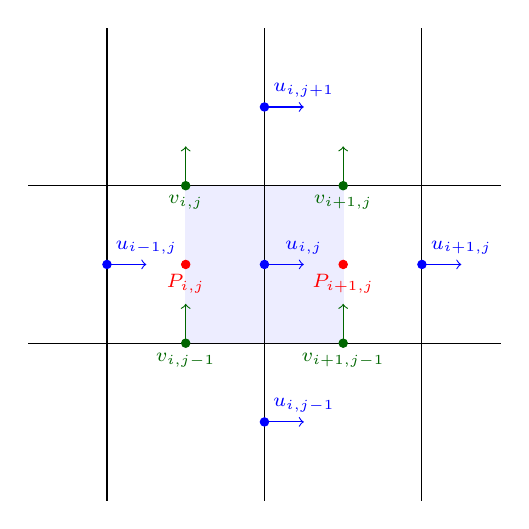
\begin{tikzpicture}[scale=1, style={font=\scriptsize}]
	\tikzset{dimen/.style={<->,>=latex,thin,every rectangle node/.style={fill=white,midway,font=\small}}}
	
	\filldraw[blue!7] (1,0) -- (3,0) -- (3,2) -- (1, 2) -- cycle;
	\draw (-1, 0) -- (5, 0);
	\draw (-1, 2) -- (5, 2);
	\draw (0, -2) -- (0, 4);
	\draw (2, -2) -- (2, 4);
	\draw (4, -2) -- (4, 4);
	
	\filldraw[red] (1, 1) circle (1.5pt);
	\filldraw[red] (3, 1) circle (1.5pt);
	\filldraw[green!40!black] (1, 2) circle (1.5pt);
	\filldraw[green!40!black] (1, 0) circle (1.5pt);
	\filldraw[green!40!black] (3, 0) circle (1.5pt);
	\filldraw[green!40!black] (3, 2) circle (1.5pt);
	\filldraw[blue] (2, 1) circle (1.5pt);
	\filldraw[blue] (4, 1) circle (1.5pt);
	\filldraw[blue] (0, 1) circle (1.5pt);
	\filldraw[blue] (2, 3) circle (1.5pt);
	\filldraw[blue] (2, -1) circle (1.5pt);
	
	\draw [->,blue] (0, 1) -- (0.5, 1);
	\draw [->,blue] (2, 1) -- (2.5, 1);
	\draw [->,blue] (4, 1) -- (4.5, 1);
	\draw [->,blue] (2, 3) -- (2.5, 3);
	\draw [->,blue] (2, -1) -- (2.5, -1);
	\draw [->,green!40!black] (1, 0) -- (1,0.5);
	\draw [->,green!40!black] (1, 2) -- (1,2.5);
	\draw [->,green!40!black] (3, 0) -- (3,0.5);
	\draw [->,green!40!black] (3, 2) -- (3,2.5);
	
	\node[below, red] at (1, 1) {$P_{i, j}$};
	\node[below, red] at (3, 1) {$P_{i+1, j}$};
	
	\node[above,blue] at (0.5, 1) {$u_{i-1,j}$};
	\node[above,blue] at (2.5, 1) {$u_{i,j}$};
	\node[above,blue] at (4.5, 1) {$u_{i+1,j}$};
	\node[above,blue] at (2.5, 3) {$u_{i,j+1}$};
	\node[above,blue] at (2.5, -1) {$u_{i,j-1}$};
	\node[below,green!40!black] at (1, 0) {$v_{i,j-1}$};
	\node[below,green!40!black] at (1, 2) {$v_{i,j}$};
	\node[below,green!40!black] at (3, 0) {$v_{i+1,j-1}$};
	\node[below,green!40!black] at (3, 2) {$v_{i+1,j}$};
	\end{tikzpicture}
	\caption{An internal $u$-velocity control volume.}
	\label{fig:CV-u}
\end{figure}

\begin{figure}[H]
	\centering
	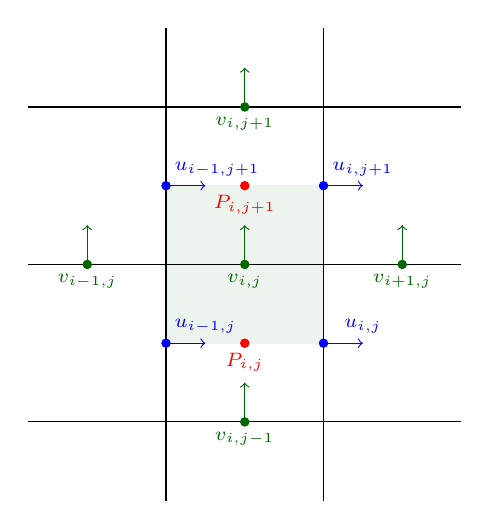
\begin{tikzpicture}[scale=1, style={font=\scriptsize}]
	\tikzset{dimen/.style={<->,>=latex,thin,every rectangle node/.style={fill=white,midway,font=\small}}}
	
	\filldraw[green!40!black!7] (0,1) -- (2,1) -- (2,3) -- (0, 3) -- cycle;
	\draw (-1.75, 0) -- (3.75, 0);
	\draw (-1.75, 2) -- (3.75, 2);
	\draw (-1.75, 4) -- (3.75, 4);
	\draw (0, -1) -- (0, 5);
	\draw (2, -1) -- (2, 5);
	
	\filldraw[red] (1, 1) circle (1.5pt);
	\filldraw[red] (1, 3) circle (1.5pt);
	\filldraw[blue] (0, 1) circle (1.5pt);
	\filldraw[blue] (2, 1) circle (1.5pt);
	\filldraw[blue] (0, 3) circle (1.5pt);
	\filldraw[blue] (2, 3) circle (1.5pt);
	\filldraw[green!40!black] (1, 0) circle (1.5pt);
	\filldraw[green!40!black] (1, 2) circle (1.5pt);
	\filldraw[green!40!black] (1, 4) circle (1.5pt);
	\filldraw[green!40!black] (-1, 2) circle (1.5pt);
	\filldraw[green!40!black] (3, 2) circle (1.5pt);
	
	\draw [->,blue] (0, 1) -- (0.5, 1);
	\draw [->,blue] (2, 1) -- (2.5, 1);
	\draw [->,blue] (0, 3) -- (0.5, 3);
	\draw [->,blue] (2, 3) -- (2.5, 3);
	\draw [->,green!40!black] (1, 0) -- (1,0.5);
	\draw [->,green!40!black] (1, 2) -- (1,2.5);
	\draw [->,green!40!black] (1, 4) -- (1, 4.5);
	\draw [->,green!40!black] (-1, 2) -- (-1, 2.5);
	\draw [->,green!40!black] (3, 2) -- (3, 2.5);
	
	\node[below, red] at (1, 1) {$P_{i, j}$};
	\node[below, red] at (1, 3) {$P_{i, j+1}$};
	\node[above,blue] at (0.5, 1) {$u_{i-1,j}$};
	\node[above,blue] at (2.5, 1) {$u_{i,j}$};
	\node[above,blue] at (0.65, 3) {$u_{i-1,j+1}$};
	\node[above,blue] at (2.5, 3) {$u_{i,j+1}$};
	\node[below,green!40!black] at (1, 2) {$v_{i,j}$};
	\node[below,green!40!black] at (1, 0) {$v_{i,j-1}$};
	\node[below,green!40!black] at (1, 4) {$v_{i,j+1}$};
	\node[below,green!40!black] at (-1, 2) {$v_{i-1,j}$};
	\node[below,green!40!black] at (3, 2) {$v_{i+1,j}$};
	\end{tikzpicture}
	\caption{An internal $v$-velocity control volume.}
	\label{fig:CV-v}
\end{figure}

\begin{figure}[H]
	\centering
	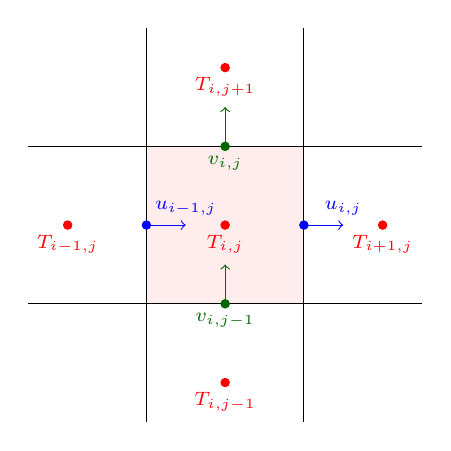
\begin{tikzpicture}[scale=1, style={font=\scriptsize}]
	\tikzset{dimen/.style={<->,>=latex,thin,every rectangle node/.style={fill=white,midway,font=\small}}}
	
	\filldraw[red!7] (0,0) -- (2,0) -- (2,2) -- (0, 2) -- cycle;
	\draw (-1.5, 0) -- (3.5, 0);
	\draw (-1.5, 2) -- (3.5, 2);
	\draw (0, -1.5) -- (0, 3.5);
	\draw (2, -1.5) -- (2, 3.5);
	
	\filldraw[red] (1, 1) circle (1.5pt);
	\filldraw[blue] (0, 1) circle (1.5pt);
	\filldraw[green!40!black] (1, 0) circle (1.5pt);
	\filldraw[blue] (2, 1) circle (1.5pt);
	\filldraw[green!40!black] (1, 2) circle (1.5pt);
	\filldraw[red] (-1, 1) circle (1.5pt);
	\filldraw[red] (3, 1) circle (1.5pt);
	\filldraw[red] (1, 3) circle (1.5pt);
	\filldraw[red] (1, -1) circle (1.5pt);
	
	\draw [->,blue] (0, 1) -- (0.5, 1);
	\draw [->,blue] (2, 1) -- (2.5, 1);
	\draw [->,green!40!black] (1, 0) -- (1,0.5);
	\draw [->,green!40!black] (1, 2) -- (1,2.5);
	
	\node[below, red] at (1, 1) {$T_{i, j}$};
	\node[below, red] at (3, 1) {$T_{i+1, j}$};
	\node[below, red] at (-1, 1) {$T_{i-1, j}$};
	\node[below, red] at (1, 3) {$T_{i, j+1}$};
	\node[below, red] at (1, -1) {$T_{i, j-1}$};
	
	\node[above,blue] at (0.5, 1) {$u_{i-1,j}$};
	\node[above,blue] at (2.5, 1) {$u_{i,j}$};
	\node[below,green!40!black] at (1, 0) {$v_{i,j-1}$};
	\node[below,green!40!black] at (1, 2) {$v_{i,j}$};
	\end{tikzpicture}
	\caption{An internal temperature control volume.}
	\label{fig:CV-T}
\end{figure}

\subsection{Velocity guess}
\label{subsec:velocity-guess}

Define the Pechlet number on each boundary of a CV for variable $\phi$ centered at node $\phi_{i,j}$ as
\begin{equation}
P^{\phi_{i,j}}_\text{bd} = \frac{F^{\phi_{i,j}}_\text{bd}}{D^{\phi_{i,j}}_\text{bd}} \,, \quad \text{where} \quad \text{bd} = [n, e, s, w] \quad \text{and} \quad \phi = [u, v]\,.
\end{equation}

The integration of the $x$ and $y$-momentum equations (generalizing again with $\phi = [u, v]$) using the power-law scheme results in the equation (for $i = 1, \ldots, M_x^\phi - 1\,\,,\, j = 1, \ldots, M_y^\phi - 1$)
\begin{subequations}
	\label{eq:power}
	\begin{align}
	a^{\phi_{i,j}}_p \phi^*_{i,j} & = a^{\phi_{i,j}}_n \phi^*_{i, j+1} + a^{\phi_{i,j}}_e \phi^*_{i+1, j} + a^{\phi_{i,j}}_s \phi^*_{i, j-1} + a^{\phi_{i,j}}_w \phi^*_{i-1, j} + a_b^{\phi_{i,j}}\,,\\
	a^{\phi_{i,j}}_n & = D^{\phi_{i,j}}_n \max \left[0, (1 - 0.1 |P^{\phi_{i,j}}_n|)^5\right] + \max \left[ -F^{\phi_{i,j}}_n, 0 \right]\,, \\
	a^{\phi_{i,j}}_e & = D^{\phi_{i,j}}_e \max \left[0, (1 - 0.1 |P^{\phi_{i,j}}_e|)^5\right] + \max \left[ -F^{\phi_{i,j}}_e, 0 \right]\,, \\
	a^{\phi_{i,j}}_s & = D^{\phi_{i,j}}_s \max \left[0, (1 - 0.1 |P^{\phi_{i,j}}_s|)^5\right] + \max \left[ F^{\phi_{i,j}}_s, 0 \right]\,, \\
	a^{\phi_{i,j}}_w & = D^{\phi_{i,j}}_w \max \left[0, (1 - 0.1 |P^{\phi_{i,j}}_w|)^5\right] + \max \left[ F^{\phi_{i,j}}_w, 0 \right]\,, \\
	a^{\phi_{i,j}}_p & = a^{\phi_{i,j}}_n + a^{\phi_{i,j}}_e + a^{\phi_{i,j}}_s + a^{\phi_{i,j}}_w\,, \\
	a^{\phi_{i,j}}_b & = \begin{cases}
	\Delta y (p^*_{i,j} - p^*_{i+1,j})\,, & \phi = u\\
	\Delta x (p^*_{i,j} - p^*_{i, j+1})\,, & \phi = v
	\end{cases}\,.
	\end{align}
\end{subequations}

\subsubsection{$u$-velocity guess update}

In all discussion that follow, we are considering a $u$-CV defined by the central node $u_{i,j}$. For simplicity we will define the width of each $u$-CV as
\begin{equation}
\Delta x^{u_{i,j}} = \begin{cases}
\Delta x\,, & 1 < i < M_x^u - 1 \\
\frac{3}{2} \Delta x\,, & \text{otherwise}
\end{cases}\,,
\end{equation}
and we will also define the $y$-distance from $u_{i,j}$ to the north and south pressure interfaces, respectively, as
\begin{subequations}
	\begin{align}
	\delta y^{u_{i,j}}_{p_n} & = \begin{cases}
	\frac{1}{2} \Delta y\,, & j = M_y^u - 1\,, \\
	\Delta y\,, & \text{otherwise}
	\end{cases}\,, \\
	\delta y^{u_{i,j}}_{p_s} & = \begin{cases}
	\frac{1}{2} \Delta y\,, & j = 1\,, \\
	\Delta y\,, & \text{otherwise}
	\end{cases}\,.
	\end{align}
\end{subequations}
The diffusion coefficients are then defined as
\begin{subequations}
	\begin{align}
	D_n^{u_{i,j}} & = \frac{\mu \Delta x^{u_{i,j}}}{\delta y^{u_{i,j}}_{p_n}}\,,\\
	D_e^{u_{i,j}} & = \frac{\mu\Delta y}{\Delta x}\,,\\
	D_s^{u_{i,j}} & = \frac{\mu \Delta x^{u_{i,j}}}{\delta y^{u_{i,j}}_{p_s}}\,,\\
	D_w^{u_{i,j}} & = \frac{\mu\Delta y}{\Delta x}\,.
	\end{align}
\end{subequations}
Lastly, the flow rates are defined as
\begin{subequations}
	\begin{align}
	F_n^{u_{i,j}} & = \rho \Delta x^{u_{i,j}} \begin{cases}
	\frac{1}{6} \left(v^*_{0, j} + 3 v^*_{1, j} + 2 v^*_{2, j} \right)\,, & i = 1 \\
	\frac{1}{6} \left(2 v^*_{i, j} + 3 v^*_{i + 1, j} + v^*_{i + 2, j} \right)\,, & i = M_x^u - 1 \\
	\frac{1}{2} \left(v^*_{i, j} + v^*_{i + 1, j}\right)\,, & \text{otherwise} 
	\end{cases}\,, \\
	F_e^{u_{i,j}} & = \rho \Delta y \begin{cases}
	u^*_{M_x^u, j}\,, & i = M_x^u - 1 \\
	\frac{1}{2} \left(u^*_{i+1, j} + u^*_{i,j}\right)\,, & \text{otherwise}
	\end{cases}\,, \\
	F_s^{u_{i,j}} & = \rho \Delta x^{u_{i,j}} \begin{cases}
	\frac{1}{6} \left(v^*_{0, j - 1} + 3 v^*_{1, j - 1} + 2 v^*_{2, j - 1} \right)\,, & i = 1 \\
	\frac{1}{6} \left(2 v^*_{i, j - 1} + 3 v^*_{i + 1, j - 1} + v^*_{i + 2, j - 1} \right)\,, & i = M_x^u - 1 \\
	\frac{1}{2} \left(v^*_{i, j - 1} + v^*_{i + 1, j - 1}\right)\,, & \text{otherwise} 
	\end{cases} \\
	F_w^{u_{i,j}} & = \rho \Delta y \begin{cases}
	u^*_{0, j}\,, & i = 1 \\
	\frac{1}{2} \left( u^*_{i - 1, j} + u^*_{i, j} \right)\,, & \text{otherwise}
	\end{cases}\,.
	\end{align}
\end{subequations}

\subsubsection{$v$-velocity guess update}

Similarly, we will consider a $v$-CV defined by the central node $v_{i,j}$. The width of each $v$-CV is defined as
\begin{equation}
\Delta y^{v_{i,j}} = \begin{cases}
\Delta y \,, & 1 < j < M_y^v - 1 \\
\frac{3}{2} \Delta y \,, & \text{otherwise}
\end{cases}\,,
\end{equation}
and we will also define the $x$-distance from $v_{i,j}$ to the east and west pressure interfaces, respectively, as
\begin{subequations}
	\begin{align}
	\delta x^{v_{i,j}}_{p_e} & = \begin{cases}
	\frac{1}{2} \Delta x\,, & i = M_x^v - 1 \\
	\Delta x \,, & \text{otherwise}
	\end{cases}\,, \\
	\delta x^{v_{i,j}}_{p_w} & = \begin{cases}
	\frac{1}{2} \Delta x\,, & i = 1\,, \\
	\Delta x\,, & \text{otherwise}
	\end{cases}\,.
	\end{align}
\end{subequations}
The diffusion coefficients are then defined as
\begin{subequations}
	\begin{align}
	D_n^{v_{i,j}} & = \frac{\mu \Delta x}{\Delta y}\,,\\
	D_e^{v_{i,j}} & = \frac{\mu \Delta y^{v_{i,j}}}{\delta x^{v_{i,j}}_{p_e}}\,,\\
	D_s^{v_{i,j}} & = \frac{\mu \Delta x}{\Delta y}\,,\\
	D_w^{v_{i,j}} & = \frac{\mu\Delta y^{v_{i,j}}}{\delta x^{v_{i,j}}_{p_w}}\,.
	\end{align}
\end{subequations}
Lastly, the flow rates are defined as
\begin{subequations}
	\begin{align}
	F_n^{v_{i,j}} & = \rho \Delta x \begin{cases}
	v^*_{i, M_y^v}\,, & j = M_y^v - 1 \\
	\frac{1}{2} \left(v^*_{i, j+1} + v^*_{i,j}\right)\,, & \text{otherwise}
	\end{cases}\,, \\
	F_e^{v_{i,j}} & = \rho \Delta y^{v_{i,j}} \begin{cases}
	\frac{1}{6} \left( u^*_{i, 0} + 3 u^*_{i, 1} + 2 u^*_{i, 2} \right)\,, & j = 1 \\
	\frac{1}{6} \left( 2 u^*_{i, j} + 3 u^*_{i, j + 1} + 2 u^*_{i, j + 2} \right)\,, & j = M_y^v - 1 \\
	\frac{1}{2} \left( u^*_{i, j} + u^*_{i, j + 1} \right)\,, & \text{otherwise} 
	\end{cases}\,, \\
	F_s^{v_{i,j}} & = \rho \Delta x \begin{cases}
	v^*_{i, 0}\,, & j = 1 \\
	\frac{1}{2} \left(v^*_{i, j+ 1} + v^*_{i,j}\right)\,, & \text{otherwise}
	\end{cases}\,, \\
	F_w^{v_{i,j}} & = \rho \Delta y^{v_{i,j}} \begin{cases}
	\frac{1}{6} \left( u^*_{i - 1, 0} + 3 u^*_{i - 1, 1} + 2 u^*_{i - 1, 2} \right)\,, & j = 1 \\
	\frac{1}{6} \left( 2 u^*_{i - 1, j} + 3 u^*_{i - 1, j + 1} + 2 u^*_{i - 1, j + 2} \right)\,, & j = M_y^v - 1 \\
	\frac{1}{2} \left( u^*_{i - 1, j} + u^*_{i - 1, j + 1} \right)\,, & \text{otherwise} 
	\end{cases}\,.
	\end{align}
\end{subequations}

\subsection{Pressure correction solve}
\label{subsec:pc-solve}

At convergence, $u' = v' = p' = 0$, therefore it is irrelevant as to how we find them. Subtracting (exact - guessed) forms of Equation \eqref{eq:power} one obtains
\begin{subequations}
	\begin{align}
	a^{u_{i,j}}_p u'_{i,j} & = a^{u_{i,j}}_n u'_{i, j+1} + a^{u_{i,j}}_e u'_{i+1, j} + a^{u_{i,j}}_s u'_{i, j-1} + a^{u_{i,j}}_w u'_{i-1, j} + \Delta y (p'_{i,j} - p'_{i+1,j}) \,, \\
	a^{v_{i,j}}_p v'_{i,j} & = a^{v_{i,j}}_n v'_{i, j+1} + a^{v_{i,j}}_e v'_{i+1, j} + a^{v_{i,j}}_s v'_{i, j-1} + a^{v_{i,j}}_w v'_{i-1, j} + \Delta x (p'_{i,j} - p'_{i, j+1}) \,.
	\end{align}
\end{subequations}
Drop the neighbor terms in the equations above (implying that velocity corrections are local) to obtain
\begin{subequations}
	\label{eq:velocity_corrector}
	\begin{align}
	u_{i,j}' & = \frac{\Delta y}{a_p^{u_{i,j}}} (p'_{i,j} - p'_{i+1,j})\,, \\
	v_{i,j}' & = \frac{\Delta x}{a_p^{v_{i,j}}} (p'_{i,j} - p'_{i, j+1})\,.
	\end{align}
\end{subequations}
Integrate the continuity equation over a $p$-CV defined by the central node $p_{i,j}$ and substitute $u = u^* + u'$, $v = v^* + v'$, and the above Equations to obtain
\begin{subequations}
	\label{eq:pc}
	\begin{align}
	a^{p'_{i,j}}_p p'_{i,j} & = a^{p'_{i,j}}_n p'_{i, j+1} + a^{p'_{i,j}}_e p'_{i+1, j} + a^{p'_{i,j}}_s p'_{i, j-1} + a^{p'_{i,j}}_w p'_{i-1, j} + a_b^{p'_{i,j}}\,,\\
	a^{p'_{i,j}}_n & = \begin{cases}
	\rho \Delta x^2 / a_p^{v_{i, j}}\,, & j < M_y^p - 1 \\
	0\,, & \text{otherwise}
	\end{cases}\,, \\
	a^{p'_{i,j}}_e & = \begin{cases}
	\rho \Delta y^2 / a_p^{u_{i, j}}\,, & i < M_x^p - 1 \\
	0\,, & \text{otherwise}
	\end{cases}\,, \\
	a^{p'_{i,j}}_s & = \begin{cases}
	\rho \Delta x^2 / a_p^{v_{i, j - 1}}\,, & j > 1 \\
	0\,, & \text{otherwise}
	\end{cases}\,, \\
	a^{p'_{i,j}}_w & = \begin{cases}
	\rho \Delta y^2 / a_p^{u_{i - 1, j}}\,, & i > 1 \\
	0\,, & \text{otherwise}
	\end{cases}\,, \\
	a^{p'_{i,j}}_p & = a^{p'_{i,j}}_n + a^{p'_{i,j}}_e + a^{p'_{i,j}}_s + a^{p'_{i,j}}_w\,, \\
	a^{p'_{i,j}}_b & = \rho \left(\Delta y (u_{i - 1, j}^* - u^*_{i,j}) + \Delta x(v^*_{i, j - 1} - v^*_{i,j})\right)\,.
	\end{align}
\end{subequations}

\subsection{Velocity and pressure correction}
\label{subsec:correction}

Lastly, the velocities are then updated using Equation \eqref{eq:velocity_corrector} with
\begin{subequations}
	\begin{align}
	u_{i,j} & = u_{i,j} + \frac{\Delta y}{a_p^{u_{i,j}}} (p'_{i,j} - p'_{i+1,j})\,,\quad i = 1, \ldots, M_x^u - 1\,, \quad j = 1, \ldots, M_y^u - 1\,, \\
	v_{i,j} & = v_{i,j} + \frac{\Delta x}{a_p^{v_{i,j}}} (p'_{i,j} - p'_{i, j+1})\,,\quad i = 1, \ldots, M_x^v - 1\,, \quad j = 1, \ldots, M_y^v - 1\,,
	\end{align}
\end{subequations}
and the pressures  (take note of the relaxation parameter $\alpha_p$) with
\begin{equation}
p_{i,j} = p_{i,j} + \alpha_p p'_{i,j} \,,\quad i = 1, \ldots, M_x^p - 1\,, \quad j = 1, \ldots, M_y^p - 1\,.
\end{equation}

\subsection{System solver}

The systems in Equations  \eqref{eq:power} and \eqref{eq:pc} are solved using the line-by-line method with TDMA as the matrix solver. In this method, a tri-diagonal system is formed as the terms from one of the dimensions are lagged. Consider the simple system
\begin{equation}
a_p^{i,j} \phi_{i,j} = a_n^{i,j} \phi_{i,j+1} + a_e^{i,j} \phi_{i+1,j} + a_s^{i,j} \phi_{i,j-1} + a_w^{i,j} \phi_{i-1,j} + a_b^{i,j}\,, \quad i = 1, \ldots, N_x\,, \quad j = 1, \ldots, N_y\,.
\end{equation}
Now, consider $\phi^*$ to be a \textit{lagged} value of $\phi$, i.e., it is known and is moved to the right hand side of each equation. In solving a single physical column $i$ using the line-by-line method, the following system is solved:
\begin{equation}
a_p^{i,j} \phi_{i,j} = a_n^{i,j} \phi_{i,j+1} + a_e^{i,j} \phi^*_{i+1,j} + a_s^{i,j} \phi_{i,j-1} + a_w^{i,j} \phi^*_{i-1,j} + a_b^{i,j}\,, \quad \quad j = 1, \ldots, N_y\,.
\end{equation}
In solving a single physical row $j$ using the line-by-line method, the following system is solved:
\begin{equation}
a_p^{i,j} \phi_{i,j} = a_n^{i,j} \phi^*_{i,j+1} + a_e^{i,j} \phi_{i+1,j} + a_s^{i,j} \phi^*_{i,j-1} + a_w^{i,j} \phi_{i-1,j} + a_b^{i,j}\,, \quad \quad i = 1, \ldots, N_x\,.
\end{equation}

\section{Results}

\subsection{Problem 3: 10 $\times$ 5 grid}

The results requested for problem 3 follow in Tables \ref{table:coarse-u}, \ref{table:coarse-p-p0}, and \ref{table:coarse-T}.

\def\arraystretch{1.3}
\begin{table}[H]
	\scriptsize
	\centering
	\caption{The $u$-velocity solution with the 10 $\times$ 5 grid. A row corresponds to a $x$-position and a column corresponds to an $y$-position.}
	\vspace{0.2cm}
	\sisetup{output-exponent-marker = \text{E}, table-format=2.5e1,group-digits=false,retain-zero-exponent=true}
	\begin{tabular}{c|S|S|S|S|S|S|S}
		& {1} & {2} & {3} & {4} & {5} & {6} & {7} \\
		\hline
		1 & 5.06931e-03 & 5.06931e-03 & 5.06931e-03 & 5.06931e-03 & 5.06931e-03 & 5.06931e-03 & 5.06931e-03 \\
		2 & 0.00000e+00 & 3.02156e-03 & 6.10805e-03 & 7.08733e-03 & 6.10805e-03 & 3.02156e-03 & 0.00000e+00 \\
		3 & 0.00000e+00 & 2.84164e-03 & 6.18930e-03 & 7.28469e-03 & 6.18930e-03 & 2.84164e-03 & 0.00000e+00 \\
		4 & 0.00000e+00 & 2.81967e-03 & 6.19551e-03 & 7.31618e-03 & 6.19551e-03 & 2.81967e-03 & 0.00000e+00 \\
		5 & 0.00000e+00 & 2.81677e-03 & 6.19585e-03 & 7.32132e-03 & 6.19585e-03 & 2.81677e-03 & 0.00000e+00 \\
		6 & 0.00000e+00 & 2.81636e-03 & 6.19583e-03 & 7.32217e-03 & 6.19583e-03 & 2.81636e-03 & 0.00000e+00 \\
		7 & 0.00000e+00 & 2.81630e-03 & 6.19583e-03 & 7.32231e-03 & 6.19583e-03 & 2.81630e-03 & 0.00000e+00 \\
		8 & 0.00000e+00 & 2.81629e-03 & 6.19582e-03 & 7.32233e-03 & 6.19582e-03 & 2.81629e-03 & 0.00000e+00 \\
		9 & 0.00000e+00 & 2.81628e-03 & 6.19582e-03 & 7.32234e-03 & 6.19582e-03 & 2.81628e-03 & 0.00000e+00 \\
		10 & 0.00000e+00 & 2.81628e-03 & 6.19582e-03 & 7.32234e-03 & 6.19582e-03 & 2.81628e-03 & 0.00000e+00 \\
		11 & 0.00000e+00 & 2.81628e-03 & 6.19582e-03 & 7.32234e-03 & 6.19582e-03 & 2.81628e-03 & 0.00000e+00 \\
	\end{tabular}
	\label{table:coarse-u}
\end{table}

\def\arraystretch{1.3}
\begin{table}[H]
	\scriptsize
	\centering
	\caption{The $(P - P_0)$ solution with the 10 $\times$ 5 grid. A row corresponds to a $x$-position and a column corresponds to an $y$-position.}
	\vspace{0.2cm}
	\sisetup{output-exponent-marker = \text{E}, table-format=2.5e1,group-digits=false,retain-zero-exponent=true}
	\begin{tabular}{c|S|S|S|S|S|S|S}
		& {1} & {2} & {3} & {4} & {5} & {6} & {7} \\
		\hline
		1 & 2.88374e-01 & 2.88374e-01 & 2.88353e-01 & 2.88346e-01 & 2.88353e-01 & 2.88374e-01 & 2.88374e-01 \\
		2 & 2.88374e-01 & 2.88374e-01 & 2.88353e-01 & 2.88346e-01 & 2.88353e-01 & 2.88374e-01 & 2.88374e-01 \\
		3 & 2.40648e-01 & 2.40648e-01 & 2.40651e-01 & 2.40653e-01 & 2.40651e-01 & 2.40648e-01 & 2.40648e-01 \\
		4 & 2.11749e-01 & 2.11749e-01 & 2.11750e-01 & 2.11750e-01 & 2.11750e-01 & 2.11749e-01 & 2.11749e-01 \\
		5 & 1.83440e-01 & 1.83440e-01 & 1.83440e-01 & 1.83440e-01 & 1.83440e-01 & 1.83440e-01 & 1.83440e-01 \\
		6 & 1.55208e-01 & 1.55208e-01 & 1.55208e-01 & 1.55208e-01 & 1.55208e-01 & 1.55208e-01 & 1.55208e-01 \\
		7 & 1.26987e-01 & 1.26987e-01 & 1.26987e-01 & 1.26987e-01 & 1.26987e-01 & 1.26987e-01 & 1.26987e-01 \\
		8 & 9.87671e-02 & 9.87671e-02 & 9.87671e-02 & 9.87671e-02 & 9.87671e-02 & 9.87671e-02 & 9.87671e-02 \\
		9 & 7.05479e-02 & 7.05479e-02 & 7.05479e-02 & 7.05479e-02 & 7.05479e-02 & 7.05479e-02 & 7.05479e-02 \\
		10 & 4.23287e-02 & 4.23287e-02 & 4.23287e-02 & 4.23287e-02 & 4.23287e-02 & 4.23287e-02 & 4.23287e-02 \\
		11 & 0.00000e+00 & 0.00000e+00 & 0.00000e+00 & 0.00000e+00 & 0.00000e+00 & 0.00000e+00 & 0.00000e+00 \\
		12 & 0.00000e+00 & 0.00000e+00 & 0.00000e+00 & 0.00000e+00 & 0.00000e+00 & 0.00000e+00 & 0.00000e+00 \\
	\end{tabular}
	\label{table:coarse-p-p0}
\end{table}

\def\arraystretch{1.3}
\begin{table}[H]
	\scriptsize
	\centering
	\caption{The $T$ solution with the 10 $\times$ 5 grid. A row corresponds to a $x$-position and a column corresponds to an $y$-position.}
	\vspace{0.2cm}
	\sisetup{table-format=2.5,group-digits=false}
	\begin{tabular}{c|S|S|S|S|S|S|S}
		& {1} & {2} & {3} & {4} & {5} & {6} & {7} \\
		\hline
		1 & 26.64204 & 25.00000 & 25.00000 & 25.00000 & 25.00000 & 25.00000 & 26.64204 \\
		2 & 27.69621 & 26.05418 & 25.36548 & 25.17769 & 25.36548 & 26.05418 & 27.69621 \\
		3 & 28.84253 & 27.20050 & 25.72681 & 25.36877 & 25.72681 & 27.20050 & 28.84253 \\
		4 & 29.72586 & 28.08382 & 26.15140 & 25.63232 & 26.15140 & 28.08382 & 29.72586 \\
		5 & 30.44158 & 28.79955 & 26.60972 & 25.95974 & 26.60972 & 28.79955 & 30.44158 \\
		6 & 31.06105 & 29.41902 & 27.08232 & 26.33547 & 27.08232 & 29.41902 & 31.06105 \\
		7 & 31.62445 & 29.98241 & 27.56009 & 26.74529 & 27.56009 & 29.98241 & 31.62445 \\
		8 & 32.15448 & 30.51244 & 28.03926 & 27.17831 & 28.03926 & 30.51244 & 32.15448 \\
		9 & 32.66429 & 31.02226 & 28.51841 & 27.62677 & 28.51841 & 31.02226 & 32.66429 \\
		10 & 33.16165 & 31.51962 & 28.99712 & 28.08535 & 28.99712 & 31.51962 & 33.16165 \\
		11 & 33.65119 & 32.00915 & 29.47532 & 28.55050 & 29.47532 & 32.00915 & 33.65119 \\
		12 & 34.14073 & 32.49869 & 29.95352 & 29.01564 & 29.95352 & 32.49869 & 34.14073 \\
	\end{tabular}
	\label{table:coarse-T}
\end{table}

\subsection{Problem 4: 180 $\times$ 54 grid}

The requirements for problem (b) part i and ii were combined into Figure \ref{fig:p2} as seen below. With increasing grid refinement, both centerline velocity profiles approached towards the reference solution obtained from Roy et. al. In addition, a once-more-refined run is compared with 256x256 CVs with good agreement.

\begin{figure}[H]
	\centering
	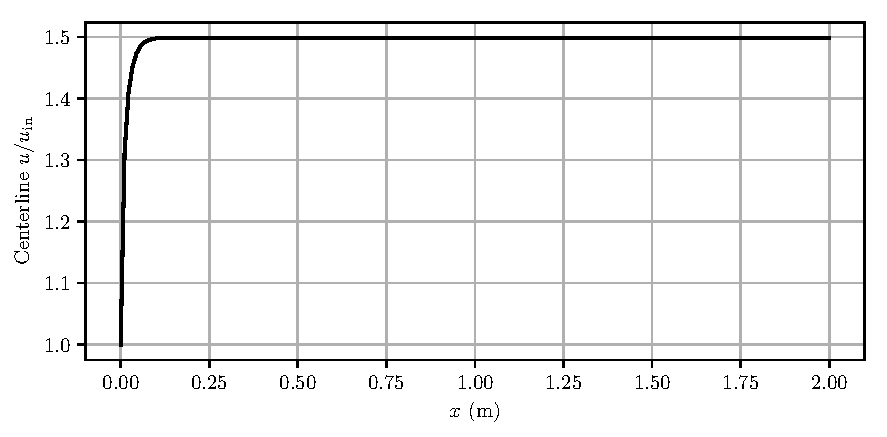
\includegraphics[width=0.75\linewidth]{../results/u_centerline}
	\caption{$u/u_\mathrm{in}$ plotted along the centerline of the channel for the 180 $\times$ 54 grid.}
	\label{fig:u-centerline}
\end{figure}

\begin{figure}[H]
	\centering
	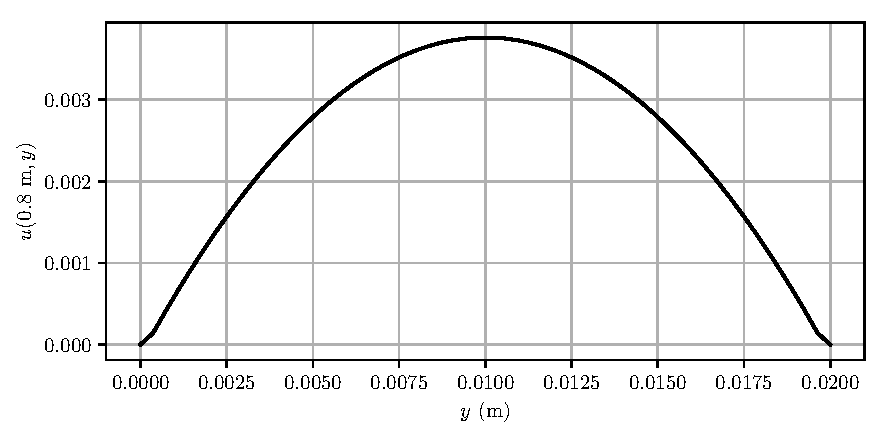
\includegraphics[width=0.75\linewidth]{../results/u_0p8}
	\caption{$u$ plotted at $x = 0.8$ m for the 180 $\times$ 54 grid.}
	\label{fig:u-0p8}
\end{figure}

\begin{figure}[H]
	\centering
	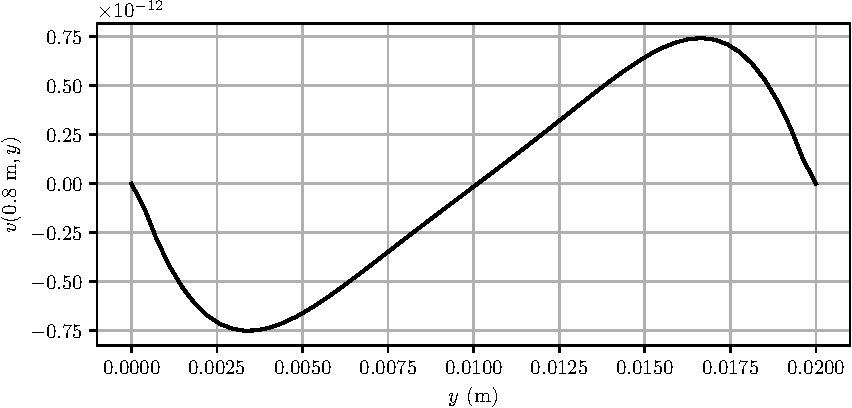
\includegraphics[width=0.75\linewidth]{../results/v_0p8}
	\caption{$v$ plotted at $x = 0.8$ m for the 180 $\times$ 54 grid.}
	\label{fig:v-0p8}
\end{figure}

\begin{figure}[H]
	\centering
	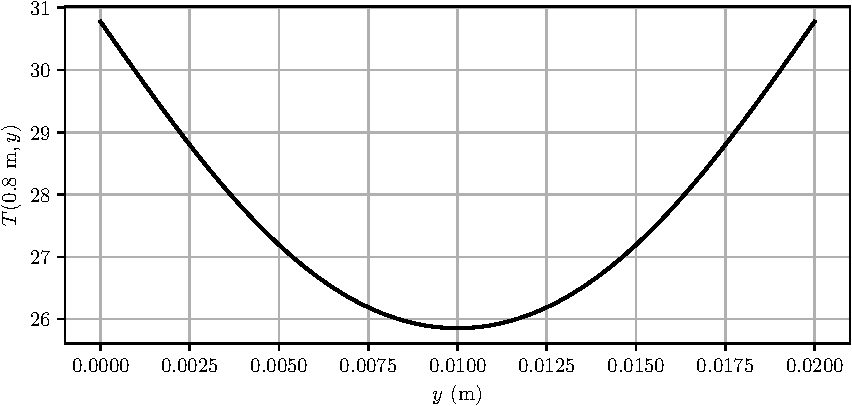
\includegraphics[width=0.75\linewidth]{../results/T_0p8}
	\caption{$T$ plotted at $x = 0.8$ m for the 180 $\times$ 54 grid.}
	\label{fig:T-0p8}
\end{figure}

\begin{figure}[H]
	\centering
	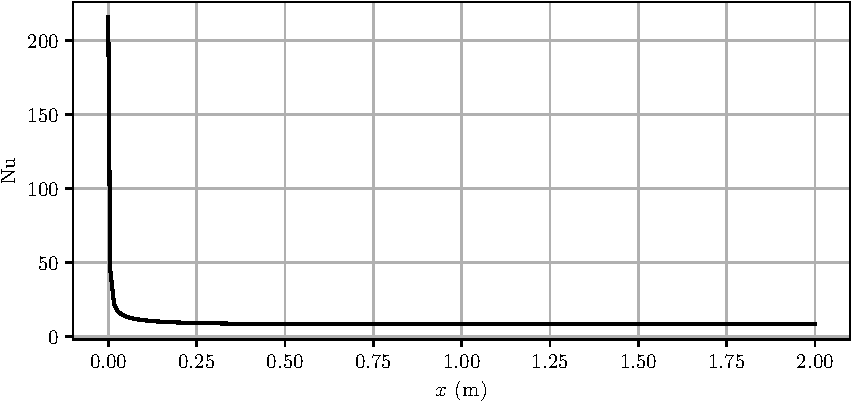
\includegraphics[width=0.75\linewidth]{../results/Nu}
	\caption{The Nusselt number plotted as a function of stream-wise distance for the 180 $\times$ 54 grid.}
	\label{fig:Nu}
\end{figure}

\section*{Code listing}

For the implementation, we have the following files:
\begin{itemize}
	\item \texttt{Makefile} -- Allows for compiling the c++ project with \texttt{make}.
	\item \texttt{hwk4.cpp} -- Contains the \texttt{main()} function that is required by C that runs the cases requested in this problem set.
	\item \texttt{Problem.h} -- Contains the header for the \texttt{Problem} class which is the main driver for a \texttt{Flow2D::Problem}.
	\item \texttt{Variable.h} -- Contains the \texttt{Flow2D::Variable} class, which is a storage container for a single variable (i.e., $u$).
	\item \texttt{Problem.cpp} -- Contains the \texttt{run()} functions that executes a \texttt{Problem}.
	\item \texttt{Problem\_coefficients.cpp} -- Contains the functions for solving coefficients in a \texttt{Problem}.
	\item \texttt{Problem\_corrections.cpp} -- Contains the functions for correcting solutions in a \texttt{Problem}.
	\item \texttt{Problem\_residuals.cpp} -- Contains the functions for computing residuals in a \texttt{Problem}.
	\item \texttt{Problem\_solvers.cpp} -- Contains the functions for sweeping and solving in a \texttt{Problem}.
	\item \texttt{Matrix.h} -- Contains the \texttt{Matrix} class which provides storage for a matrix with various standard matrix operations.
	\item \texttt{TriDiagonal.h} -- Contains the \texttt{TriDiagonal} class which provides storage for a tri-diagonal matrix including the TDMA solver found in the member function \texttt{solveTDMA()}.
	\item \texttt{Vector.h} -- Contains the \texttt{Vector} class for one-dimensional vector storage.
	\item \texttt{postprocess.py} - Produces the plots and tables in this report.
\end{itemize}

\subsection*{Makefile}
\inputminted[fontsize=\scriptsize]{Makefile}{../Makefile}

\subsection*{hwk5.cpp}
\inputminted[fontsize=\scriptsize]{c++}{../hwk5.cpp}

\newpage
\subsection*{Problem.h}
\inputminted[fontsize=\scriptsize]{c++}{../Problem.h}

\newpage
\subsection*{Variable.h}
\inputminted[fontsize=\scriptsize]{c++}{../Variable.h}

\newpage
\subsection*{Problem.cpp}
\inputminted[fontsize=\scriptsize]{c++}{../Problem.cpp}

\newpage
\subsection*{Problem\_coefficients.cpp}
\inputminted[fontsize=\scriptsize]{c++}{../Problem_coefficients.cpp}

\newpage
\subsection*{Problem\_corrections.cpp}
\inputminted[fontsize=\scriptsize]{c++}{../Problem_corrections.cpp}

\newpage
\subsection*{Problem\_residuals.cpp}
\inputminted[fontsize=\scriptsize]{c++}{../Problem_residuals.cpp}

\newpage
\subsection*{Problem\_solvers.cpp}
\inputminted[fontsize=\scriptsize]{c++}{../Problem_solvers.cpp}

\newpage
\subsection*{Matrix.h}
\inputminted[fontsize=\scriptsize]{c++}{../Matrix.h}

\newpage
\subsection*{TriDiagonal.h}
\inputminted[fontsize=\scriptsize]{c++}{../TriDiagonal.h}

\newpage
\subsection*{Vector.h}
\inputminted[fontsize=\scriptsize]{c++}{../Vector.h}

\newpage
\subsection*{postprocess.py}
\inputminted[fontsize=\scriptsize]{python}{../postprocess.py}

\end{document}
